\documentclass[a4paper,11pt]{article}
\usepackage{xcolor}
\usepackage{geometry}
\usepackage{hyperref}
\hypersetup{
    colorlinks=false,
    linkcolor=blue,
    linkbordercolor=blue,
    pdfborderstyle={/S/U/W 1}
}
\usepackage{graphicx}
\usepackage{float}
\usepackage[strict]{changepage} %allows indented blocks
\usepackage{amsmath}
\geometry{
a4paper,
total={170mm,257mm},
left=20mm,
top=20mm,
marginparsep=0mm,
}
\setlength\parindent{0pt} % get rid of the stupid indent

\title{Networks Cheatsheet}
\author{Thomas Boxall\\ \texttt{up2108121@myport.ac.uk}}
\date{May 2023}

\usepackage{fancyhdr}
\pagestyle{fancy}
\fancyhead{} % clear all header fields
\renewcommand{\headrulewidth}{0pt} % no line in header area
\fancyfoot{} % clear all footer fields
\renewcommand{\footrulewidth}{0.4pt}
\fancyfoot[C]{\thepage} % page number in centre of the page
\fancyfoot[R]{\footnotesize Thomas Boxall\\ \texttt{up2108121@myport.ac.uk}} % right hand footer has author name on top line and author contact on bottom line
\fancyfoot[L]{\footnotesize Networks \\ May 2023} % left hand footer has title of document on top line and date on bottom line


\begin{document}

\maketitle
\thispagestyle{fancy}

\section{Protocols}
\textbf{Protocol} is a standard method or format for communication between network devices.\\
\textbf{What-If? Conditions} are covered by protocols. Protocols allow smooth recovery from if something goes wrong (e.g. What if a packet gets corrupt? What if the communication medium fails?)\\
\textbf{Connection Oriented Protocols} operate on connections which use virtual circuits which work like a old-style landline telephone where a dedicated connection between sender and receiver is established for the duration of the transmission then torn down after the transmission is complete. This provides a good Quality of Service (QoS) however they take time to setup and teardown, and while in use no other transmission are able to use that communication link.\\
\textbf{Connectionless Protocols} operate on general transmission mediums, a bit like how the postal system works (letters/ packets move from sorting office to sorting office/ switch or router to switch or router until it arrives at the destination). The sender sends the data to transmit into the network and hopes it arrives at the receiver. These are much more efficient than connection-oriented which makes them better for situations where the throughput of data is very important (e.g. audio/ video). However, the packets may get lost, or all go different routes and arrive in the wrong order - TCP is used here to solve this.\\
\textbf{TCP/IP} (Transmission Control Protocol/ Internet Protocol) is a collection of protocols that control how data travels from one machine to another across networks.
\begin{adjustwidth}{2em}{1em}
\textit{TCP} is connection-oriented and ensures reliable data delivery through sequencing, checksum and provides flow control. At the sending device, TCP breaks the data to send into packets which the network can handle then at the recipient, TCP examines all the packets to ensure they have all arrived and are all un-corrupt then reports the status back to the sender node so it knows if it needs to retransmit any of them, finally it will reassemble the packets into the data.\\
\textit{IP} is used to envelope the data, providing a location where the sender and destination IP addresses can be added to the packet.
\end{adjustwidth}
\textbf{UDP} (User Datagram Protocol) is a connectionless transport service (there is no guarantee the packets will arrive), it provides no error checking or sequencing. UDP is much more efficient than TCP.\\
\textbf{CSMA/CD} (Carrier Sense Multi Access/ Collision Detection) is an algorithm used on Bus Topologies which detects collisions and determines how to recover from them. The way it works can be seen in Figure \ref*{fig:csmacd}. 

\begin{figure}[ht]
    \centering
    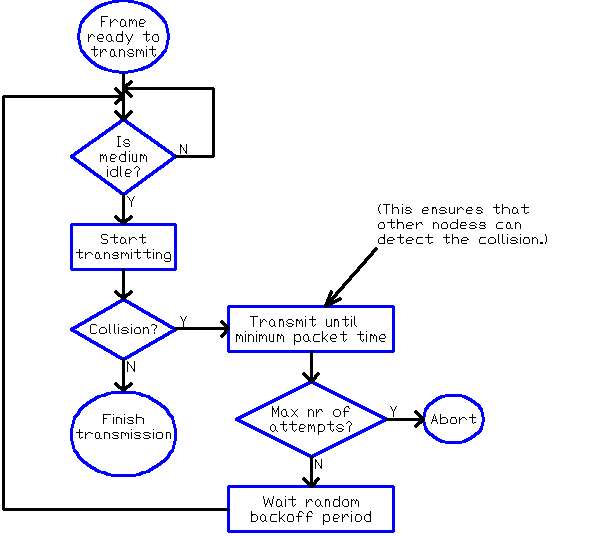
\includegraphics[width=0.8\textwidth]{../assets/csmacd.png}
    \caption{CSMA/CD Algorithm}
    \label{fig:csmacd}
\end{figure}

\section{Packets}
\textbf{Packets} are single units of data to be sent across a network. Data to be transmitted is broken into multiple packets.\\
\textbf{Packet Headers} contain the sender and recipient IP addresses.\\
\textbf{Routes} the packets takes are determined by routers. They control where the packet ``hops''. 

\section{Internet Protocol}
\textbf{Internet Protocol} (IP) is a connectionless protocol with best-effort delivery. It uses IP addresses.\\
\textbf{IP Address} is an identifier used to identify individual computers. They can either be statically assigned or dynamically assigned (this is done through DHCP) to a device.\\
\textbf{Subnet Mask} of an IP address is a 32-bit pattern used to identify the network and host address. Devices can have the same subnet mask as each other.\\
\textbf{IPv4} is the `original' format of IP addresses. It uses 32 bits.\\
\textbf{IPv6} is the `new' format of IP addresses as there were not enough in IPv4 for all devices. It uses 128 bits. 

\section{Network Capacity}
\textbf{Bandwidth} is the maximum rate of data transfer across a given path.\\
\textbf{Data rate} can be calculated using the following formula:
\begin{align*}
\mathrm{data\ rate\ (bytes/s)} &= \frac{1}{\mathrm{time\ interval\ of\ packet\ being\ sent}} \times \mathrm{packet\ size\ (bytes)}\\
\mathrm{data\ rate\ (bits/s)} &= \frac{\mathrm{data\ rate\ (bytes/s)}}{8}\\
\mathrm{data\ rate\ (kilobits/s)} &= \frac{\mathrm{data\ rate\ (bits/s)}}{1000}\\
\end{align*}

\section{Interconnection Components}
\textbf{Switches} examine the header of the packet as it arrives into the switch. The packet is forwarded to only the next node in its journey (this may be multiple places, in which case multicast is used). Switches can either operate in store and forward (where they temporarily hold the frame while making the decision about its destination) or cut through (where they start to forward the frame as soon as the destination IP address is read - requires switch and device to have same data rate).\\
\textbf{Hubs} transmit the packets to all of the connected devices, even if the packet isn't destined for that device. It is up to the device to check the recipient IP address and if it doesn't match its then the packet gets discarded.\\
\textbf{VLAN} (Virtual Local Area Network) are software which virtually divides a LAN into smaller LANs. Membership of a VLAN is set by the network admin and can be based off of which port on a switch the device connects to, MAC addresses, or a Layer 3 protocol (e.g. IP or IPX). 

\section{Standards}
\textbf{Standards} are documented agreements containing technical specifications or other precise criteria that stipulate how a particular product or service should be designed or performed. They exist outside of networking too.\\
\textbf{Standardisation Bodies} are the organisations which produce standards. Examples include IEEE (LAN standards), IEFT (Internet RFCs), ETSI (Eurpoean Telecoms), EIA/TIA (Cable standards i.e. CAT5/5e), ITU-T (Telecom \& data comms standards).  

\section{OSI Reference Model}
\textbf{Overview} The Open Systems Interconnection (OSI) reference model is based on a series of 7 layers. The data to be transmitted travels down through the seven layers to the transmission medium where it crosses the transmission medium and on the receiving device, the data climbs back up the seven layers.\\
\textbf{Layers} each have a specific function/ task. They each provide a service to the layer above. The four lower layers are concerned with the flow of data from end to end. The upper four layers are focused more towards services to the application. Layer 1 is closest to the transmission medium and layer 7 is closest to the application.
\begin{adjustwidth}{2em}{1em} 
\textit{Layer 1: Physical} is concerned with the physical characteristics of the transmission medium. It deals with voltage levels, timing of voltage changes, physical data rates, maximum transmission distances and physical connectors.\\
\textit{Layer 2: Data Link} provides access to the networking media and physical layer. It handles the transmission of the data across the medium to the intended destination. It uses MAC addresses to identify different stations on the same medium. It is concerned with network topology, network access, error notification, ordered delivery of frames, flow control. Protocols used include Ethernet, frame relay and FDDI. \\
\textit{Layer 3: Network} is concerned with the end-to-end delivery of packets. It defines the logical address \& how routing works. It also defines how to fragment packets into smaller packets to accommodate different media and its where routers operate. 

\end{adjustwidth}

\end{document}